\documentclass[10pt,conference]{IEEEtran}
\usepackage{amsmath,amssymb,booktabs,graphicx,cite}
\usepackage{tikz}
\usetikzlibrary{arrows.meta,positioning}
\usepackage{flushend}
\usepackage[hidelinks]{hyperref}
\newtheorem{proposition}{Proposition}
\newtheorem{theorem}{Theorem}
\newtheorem{corollary}{Corollary}
\newcommand{\E}{\mathbb E}
\newcommand{\Dgm}{\operatorname{Dgm}}
\newcommand{\Aut}{\operatorname{Aut}}
\newcommand{\Inf}{\operatorname{Inf}}
\title{Variational Topology for Semantic Channel Representations: Relation Functionals, Critical Loads and Resource Cost}
\author{} % Insert the author block appropriate to the selected conference.
\begin{document}
\maketitle
\begin{abstract}
A persistence diagram can survive transmission even when the receiver connects the wrong pair of named locations. We treat the connectivity that a semantic image link must preserve as a variational problem. The relation functional is the probability that a connectivity query between two named locations is answered differently on the source and on the reconstruction. We derive its first variation exactly. Near a generic score field it is a weighted $\ell^1$ norm whose weights, the critical loads, count the location pairs that each pixel connects and follow from one union--find sweep. For binary images the variation is a pixel influence. Diagram functionals are constant on orbits of the readout-graph automorphisms and move only critical vertices. On an orbit the relation rate--distortion function has a closed form and reaches three bits on the square grid, where the diagram rate is zero. A converse ties many queries to one transmission, and the variation yields a power allocation in closed form. On 320 real Omniglot glyphs, reflection preserves every diagram and changes 77.82\% of foreground query answers, five percent of the pixels carry 65.6\% of the influence, and an influence-weighted BPSK allocation lowers the relation risk at 6~dB to 3.6\% of its uniform-power value while more than doubling the pixel error rate. In a converged learned codec the same functional used as a training loss lowers the risk by only one to two percent.
\end{abstract}
\begin{IEEEkeywords}
Calculus of variations, connectivity, joint source--channel coding, persistent homology, rate--distortion theory, semantic communication.
\end{IEEEkeywords}

\section{Introduction}
A map receiver may need to decide whether two marked locations lie on the same route. A glyph receiver may need to determine whether two strokes meet. The number and lifetimes of connected components give global information in either case. They do not identify which marked locations belong to each component. The distinction matters when the encoder must use a fixed number of noisy symbols, because the receiver can produce a structurally plausible image yet answer a particular question incorrectly.

Deep joint source--channel coding (DeepJSCC) learns an image-to-symbol map and decoder through a physical channel \cite{bourtsoulatze2019deep}. TopoJSCC adds image-space cubical persistence and batchwise latent Vietoris--Rips persistence \cite{erak2026topojscc}, TopoCode uses persistence descriptors as side information \cite{guo2025topocodetopologicallyinformederror}, and topological autoencoders match critical edges of finite metric spaces \cite{moor2020topological}. Maximin affinity learning supervises connectivity through path bottlenecks \cite{turaga2009malis}. Semantic rate--distortion models place the fidelity criterion on a task variable \cite{liu2022indirect,Stavrou_2023}. Persistence-based functionals do admit a first variation, in which each diagram point moves with the value of its critical simplex \cite{carriere2021optimizing}. As a variational principle for communication they have three limits. They are constant on symmetry orbits of the readout. They give every merge event the same weight, whatever the number of location pairs that depend on it. On a latent batch they describe a sample and not an identified manifold. We therefore take as the functional the disagreement of connectivity answers between named locations, which is aware of identity, weights each event by the pairs it affects, and is evaluated through a fixed readout without a known atlas or genus. Our contributions are as follows.
\begin{itemize}
\item \emph{Functional and variation.} The relation functional and its exact threshold-integrated form (Proposition~\ref{prop:risk}), its first variation at generic fields through critical loads (Theorem~\ref{thm:loads}), and directional derivatives and pixel influences in general (Proposition~\ref{prop:influence}).
\item \emph{What diagrams forget.} Invariance of diagram functionals on automorphism orbits (Proposition~\ref{prop:aut}) and a closed-form relation rate--distortion function on an orbit (Theorem~\ref{thm:orbit}).
\item \emph{Resources.} A converse for many queries on one transmission with fading corollaries (Theorem~\ref{thm:converse}), and a variational power allocation in closed form (Proposition~\ref{prop:alloc}).
\item \emph{Evidence.} Exact counts on real glyphs for the orbit rates, the influence maps and the first-order law, an uncoded allocation experiment with three controls, and a converged learned codec on three seeds.
\end{itemize}

\section{System Model and Problem Formulation}
\subsection{Wireless image link}
Fig.~\ref{fig:system} shows the link. A source image $X\in[0,1]^{H\times W}$ has $n=HW$ pixels. An encoder maps $X$ to $k$ complex symbols $Z$ with $\|Z\|^2=k$, and the bandwidth ratio is $\rho=k/n$. The receiver observes
\begin{equation}
 V=(Y,h),\qquad Y=hZ+N,\quad N\sim\mathcal{CN}(0,\sigma^2I_k),
\end{equation}
and the signal-to-noise ratio per complex symbol is $1/\sigma^2$. AWGN has $h=1$. Coherent block Rayleigh fading draws one $h\sim\mathcal{CN}(0,1)$ per image, known to the receiver only. A decoder returns $\hat X$ from $V$. The functional, its variation and the converse below hold for every such pair. Two instances are evaluated.

\emph{Per-location link.} The image is binary, $k=n$, and pixel $v$ is sent as one BPSK symbol with power $p_v>0$, $\sum_vp_v=n$. The receiver takes the sign of each symbol. The only design variable is the allocation $p$, which may depend on the image, and the detector does not need to know it.

\emph{Learned codec.} A convolutional encoder $f_\theta$ produces $k=\rho n$ symbols in $J$ groups of lengths $k_j$. Each group is normalized to unit mean energy for every image and scaled by a power $p_j>0$, shared by all images, with $\sum_jk_jp_j=k$. The decoder $g_\phi$ reconstructs $\hat X=g_\phi(\tilde Z)$ from $\tilde Z=Y$ in AWGN and from the linear MMSE scaling $\tilde Z=h^*Y/(|h|^2+\sigma^2)$ under fading.
\begin{figure}[t]\centering
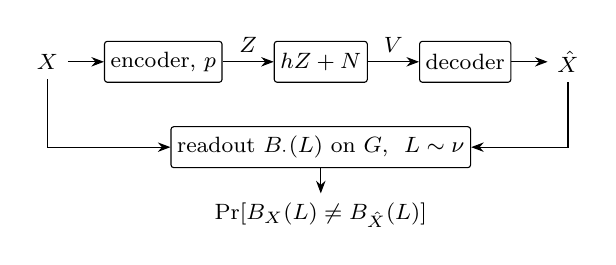
\begin{tikzpicture}[font=\footnotesize,>={Stealth[length=1.6mm]},
 box/.style={draw,rounded corners=1pt,minimum height=5.2mm,inner sep=2.2pt},node distance=4.6mm]
\node (x) {$X$};
\node[box,right=of x] (enc) {encoder, $p$};
\node[box,right=6.5mm of enc] (ch) {$hZ+N$};
\node[box,right=6.5mm of ch] (dec) {decoder};
\node[right=of dec] (xh) {$\hat X$};
\node[box,below=5.5mm of ch] (ev) {readout $B_{\cdot}(L)$ on $G$,\ \ $L\sim\nu$};
\draw[->] (x)--(enc);
\draw[->] (enc)--node[above]{$Z$}(ch);
\draw[->] (ch)--node[above]{$V$}(dec);
\draw[->] (dec)--(xh);
\draw[->] (x) |- (ev);
\draw[->] (xh) |- (ev);
\node[below=3.2mm of ev] (risk) {$\Pr[B_X(L)\ne B_{\hat X}(L)]$};
\draw[->] (ev)--(risk);
\end{tikzpicture}
\caption{Semantic image link with $k$ channel uses. The evaluator applies the same named queries to the source and to the reconstruction. Queries are never sent to the decoder.}
\label{fig:system}\end{figure}

\subsection{Shared readout and relation functional}
The knowledge shared by both terminals is a fixed aligned graph $G=(\mathcal V,\mathcal E)$, here the connected image grid with four-neighbor adjacency, and a law $\nu$ on queries $L=(a,b,t)$ in which the threshold $t$ is independent of the endpoints. The score $f_X(v)=1-X(v)$ activates high-intensity strokes or roads early. The answer $B_X(L)$ is one when $a,b$ belong to the same component of the subgraph induced on $\{f_X\le t\}$. Inactive endpoints give answer zero, and for $a=b$ the answer records whether that vertex is active.

When $\nu$ does not depend on the source, the \emph{relation functional}
\begin{equation}
 \mathcal R[\hat f;f]=d_\nu(f,\hat f)=\Pr_{L\sim\nu}\big[B_f(L)\ne B_{\hat f}(L)\big]
\end{equation}
is the $L^1(\nu)$ distance between the answer functions of two score fields and is a pseudometric. Its pullback through a decoder, $(z,z')\mapsto d_\nu(g_\phi(z),g_\phi(z'))$, is a relation pseudometric on a learned representation and is defined without inferring the homology of that representation from a finite batch. Theorem~\ref{thm:loads} shows that it is locally a weighted $\ell^1$ norm and not a Riemannian metric. A source-conditioned foreground law defines a directed loss and need not give a pseudometric.

\subsection{Three distortions and the design problem}
A code induces the pixel distortion $D_{\rm pix}=\E\|X-\hat X\|_2^2/n$, a diagram distortion $D_{\rm dgm}$ that compares unlabelled persistence diagrams of $f_X$ and $f_{\hat X}$, and the relation distortion $D_{\rm rel}=\E\,\mathcal R[f_{\hat X};f_X]$. The query, the diagrams and the foreground mask are available to the evaluator during learning or measurement and are never sent as side information. The variational design problem at fixed $k$ is
\begin{equation}
 \min\ D_{\rm pix}+\lambda_QD_{\rm rel}+\lambda_M\E L_{\rm edge}
 \quad\text{s.t.}\ \|Z\|^2=k, \label{eq:problem}
\end{equation}
over the free parameters of the link. For the per-location link these are the powers and the problem is solved in closed form to first order (Proposition~\ref{prop:alloc}). For the learned codec they are $(\theta,\phi,p)$, and $L_{\rm edge}$ is the critical-edge regularizer of Section~\ref{sec:train}.

\section{The Relation Functional and Its First Variation}
\subsection{Integrating the threshold exactly}
Define the merge level
\begin{equation}
 m_f(a,b)=\min_{\pi:a\leadsto b}\max_{v\in\pi} f(v),
\end{equation}
where the path includes both endpoints, so $m_f(a,a)=f(a)$.
\begin{proposition}\label{prop:risk}
Let the threshold have a continuous CDF $F$. For fixed endpoints the two answers disagree with probability
\begin{equation}
 |F(m_f(a,b))-F(m_{\hat f}(a,b))|, \label{eq:risk}
\end{equation}
so $\mathcal R[\hat f;f]=\E_{(a,b)}|F(m_f)-F(m_{\hat f})|$. Moreover $|m_f-m_{\hat f}|\le\|f-\hat f\|_\infty$.
\end{proposition}
\begin{IEEEproof}
A path is active at threshold $t$ precisely when its maximum score is at most $t$, so $B_f=\mathbf 1\{m_f\le t\}$. The answers disagree on the half-open interval between the merge levels. Perturbing $f$ by at most $\epsilon$ in sup norm changes the maximum on each path by at most $\epsilon$, and taking minima in both directions proves the stability statement.
\end{IEEEproof}
A uniform threshold on $[0,1]$ turns \eqref{eq:risk} into $|m_f-m_{\hat f}|$. The risk splits as $[F(m_{\hat f})-F(m_f)]_++[F(m_f)-F(m_{\hat f})]_+$, the probabilities that the receiver separates a connected pair and joins a separated pair, which can be weighted differently. With edge weights $\max(f(u),f(v))$, the heaviest edge on the path of any minimum spanning tree (MST) realizes the minimax value, so one tree serves all pairs of an image.

\subsection{Critical loads at a generic field}
Let $f$ be injective on $\mathcal V$ with smallest gap $\gamma_f$ between two values. Activate the vertices in increasing order of $f$. When $v$ enters it joins the existing components that contain its neighbors, of sizes $n_{v,1},n_{v,2},\dots$, into one component of size $N_v=1+\sum_jn_{v,j}$. Every pair $(a,b)$ is connected for the first time by exactly one vertex $v^\star(a,b)$, and $m_f(a,b)=f(v^\star(a,b))$. The \emph{critical load} of $v$ is the probability $c_f(v)$ that $v^\star(a,b)=v$ for an endpoint pair drawn from $\nu$.
\begin{theorem}[First variation at a generic field]\label{thm:loads}
(i) $\sum_vc_f(v)=1$, and for uniform ordered pairs with replacement
\begin{equation}
 c_f(v)=\big(N_v^2-\textstyle\sum_jn_{v,j}^2\big)/n^2 . \label{eq:load}
\end{equation}
(ii) If $\|\delta\|_\infty<\gamma_f/2$, then
\begin{equation}
 \mathcal R[f+\delta;f]=\sum_{v\in\mathcal V}c_f(v)\,\big|F(f(v)+\delta(v))-F(f(v))\big|, \label{eq:l1}
\end{equation}
which is $\sum_vc_f(v)|\delta(v)|$ for a uniform threshold. (iii) For generic $\hat f$ and a uniform threshold, wherever $m_{\hat f}\ne m_f$ on the support of $\nu$,
\begin{equation}
 \frac{\partial\mathcal R[\hat f;f]}{\partial\hat f(v)}=\E\big[\operatorname{sgn}(m_{\hat f}-m_f)\,\mathbf 1\{v^\star_{\hat f}(a,b)=v\}\big], \label{eq:grad}
\end{equation}
and the $\ell^1$ norm of this gradient is at most one.
\end{theorem}
\begin{IEEEproof}
(i) A pair is first connected at the level $m_f(a,b)$, which is the value of a single vertex by injectivity, and $G$ is connected. The pairs first connected by $v$ are those inside its new component that were not inside one earlier component. (ii) A perturbation below half the gap preserves the order of the values, hence the whole activation sequence and the map $v^\star$. Thus $m_{f+\delta}(a,b)=f(v^\star)+\delta(v^\star)$, and Proposition~\ref{prop:risk} gives \eqref{eq:l1}. (iii) The same argument at $\hat f$ gives $\partial m_{\hat f}(a,b)/\partial\hat f(v)=\mathbf 1\{v^\star_{\hat f}(a,b)=v\}$.
\end{IEEEproof}
Locally the relation pseudometric is therefore a weighted $\ell^1$ norm with weights read off the merge tree, and one union--find sweep computes them. The functional has a kink at the reference, which is why small perturbations cost in proportion to their size and not to its square. Equation \eqref{eq:grad} is the gradient that the MST walk of Section~\ref{sec:train} computes on sampled pairs.

The sublevel $H_0$ diagram of $f$ consists of the values at local minima and at the vertices that merge two or more components. A diagram functional moves each such value with a weight that ignores $n_{v,1}n_{v,2}$, and it has zero variation at every other vertex. The loads \eqref{eq:load} are positive at every vertex. A vertex that extends one component by itself has load $(2n_{v,1}+1)/n^2$, and a merge vertex is weighted by the number of location pairs that it connects.

\subsection{General variation and pixel influence}
\begin{proposition}\label{prop:influence}
(i) For any $f$ and direction $\delta$, the one-sided derivative of the merge level is
\begin{equation}
 m_f'(a,b;\delta)=\min_{\pi\in\Pi^\star(a,b)}\ \max_{v\in\pi:\,f(v)=m_f(a,b)}\delta(v),
\end{equation}
with $\Pi^\star(a,b)$ the minimax-optimal paths. (ii) For a binary image $x$ let $\Inf_x(v)=d_\nu(x,x\oplus e_v)$ be the relation distance to the image with pixel $v$ flipped. If the pixels flip independently with probabilities $\varepsilon_v$, $S=\sum_v\varepsilon_v$ and $\Lambda=\sum_v\varepsilon_v\Inf_x(v)$, then
\begin{equation}
 -S\Lambda\ \le\ \E\,d_\nu(x,x\oplus Z)-\Lambda\ \le\ S^2/2 . \label{eq:firstorder}
\end{equation}
\end{proposition}
\begin{IEEEproof}
(i) $m_f$ is a minimum over finitely many paths of maxima of coordinates, and the directional derivative of a finite maximum (minimum) is the maximum (minimum) over its active terms. (ii) The event that only $v$ flips has probability between $\varepsilon_v(1-S)$ and $\varepsilon_v$. Two or more flips occur with probability at most $S^2/2$, and $d_\nu\le1$.
\end{IEEEproof}
Erasing a stroke pixel separates the pairs that it joined, so cut pixels have large influence. A background pixel next to the ink joins or extends the components that it touches, and an isolated one only becomes active itself, with influence $1/n^2$ under uniform pairs. The bound \eqref{eq:firstorder} is a worst case over images.

\section{What Diagrams Forget}
Let $\Aut(G)$ be the automorphism group of the readout graph and $(f\circ\sigma)(v)=f(\sigma v)$. The square grid has the eight symmetries of the dihedral group.
\begin{proposition}\label{prop:aut}
(i) The merge level is symmetric and satisfies $f(a)=m_f(a,a)\le m_f(a,b)$ and $m_f(a,c)\le\max\{m_f(a,b),m_f(b,c)\}$. The sublevel $H_0$ diagram of $f$ is a function of the array $m_f$ that is invariant under relabelling both arguments by any permutation of $\mathcal V$. (ii) For $\sigma\in\Aut(G)$, $m_{f\circ\sigma}(a,b)=m_f(\sigma a,\sigma b)$ and $B_{f\circ\sigma}(a,b,t)=B_f(\sigma a,\sigma b,t)$, and all unlabelled persistence diagrams of $f\circ\sigma$ and $f$ coincide for every complex on which $\sigma$ acts, such as the clique complex of $G$ or the cubical complex of the pixel grid.
\end{proposition}
\begin{IEEEproof}
Concatenating two paths gives the strong triangle inequality. At level $t$ the components are the classes of $m_f(a,b)\le t$ on $\{a:m_f(a,a)\le t\}$. The array therefore determines the merge tree and, by the elder rule, the diagram. A relabelling renames only the leaves. An automorphism maps paths from $a$ to $b$ onto paths from $\sigma a$ to $\sigma b$ and preserves their maxima. It also restricts to isomorphisms of all sublevel complexes that commute with inclusions, so the persistence modules are isomorphic in every degree.
\end{IEEEproof}
Every diagram functional therefore vanishes between $f$ and $f\circ\sigma$, while $\mathcal R[f\circ\sigma;f]=\E|F(m_f(a,b))-F(m_f(\sigma a,\sigma b))|$ vanishes only if the merge function is $\sigma$-invariant almost surely.

Let $\Gamma\le\Aut(G)$ and let $\mathcal O=\{x\circ\gamma:\gamma\in\Gamma\}$ be the orbit of a template $x$, with $K=|\mathcal O|$. Assume that $\nu$ is independent of the source and invariant under $(a,b,t)\mapsto(\gamma a,\gamma b,t)$, as for uniform vertex pairs. Let $\varrho_1,\ldots,\varrho_K$ be the values $d_\nu(x,x')$, $x'\in\mathcal O$.
\begin{theorem}[Orbit rate--distortion]\label{thm:orbit}
Let $X$ be uniform on $\mathcal O$ and restrict reproductions to $\mathcal O$. Put $\delta_{\max}=K^{-1}\sum_i\varrho_i$. The minimum information for relation distortion at most $\delta$ is, in bits,
\begin{equation}
 R_Q(\delta)=\log_2K-H_2(P_\beta),\qquad 0\le\delta<\delta_{\max}, \label{eq:orbit}
\end{equation}
where $P_\beta(i)\propto2^{-\beta\varrho_i}$ and $\beta\in(0,\infty]$ solves $\sum_iP_\beta(i)\varrho_i=\delta$. For $\delta\ge\delta_{\max}$, $R_Q(\delta)=0$. Every distortion that depends only on unlabelled persistence diagrams is identically zero on $\mathcal O$ and has zero rate.
\end{theorem}
\begin{IEEEproof}
Invariance of $\nu$ and Proposition~\ref{prop:aut} give $d_\nu(g\circ\tau,g'\circ\tau)=d_\nu(g,g')$ for $\tau\in\Gamma$. Since $\Gamma$ permutes $\mathcal O$ transitively, every row and, by symmetry of $d_\nu$, every column of the distortion matrix on $\mathcal O$ is a permutation of $(\varrho_i)$. Let $\varphi(\delta)$ be the maximum entropy of a law $P$ on $K$ points with $\sum_iP(i)\varrho_i\le\delta$. It is concave, nondecreasing, and equal to $H_2(P_\beta)$ below $\delta_{\max}$. Given $\hat X=\hat x$ with conditional distortion $\delta_{\hat x}$, the conditional entropy of $X$ is at most $\varphi(\delta_{\hat x})$, so $I_2(X;\hat X)\ge\log_2K-\varphi(\delta)$ by Jensen's inequality. For achievability draw $\hat X$ uniformly and set $P(x\mid\hat x)\propto2^{-\beta d_\nu(x,\hat x)}$. The normalizer is the same in every column, and the row property makes $X$ uniform. The diagram claim is Proposition~\ref{prop:aut}.
\end{IEEEproof}
\begin{corollary}\label{cor:binary}
For two equally probable templates related by a reflection with $\alpha=d_\nu(x_0,x_1)>0$,
\begin{equation}
 R_Q(\delta)=
 \begin{cases}
 1-h_2(\delta/\alpha),&0\le\delta<\alpha/2,\\
 0,&\delta\ge\alpha/2 .
 \end{cases} \label{eq:binary}
\end{equation}
\end{corollary}
With a trivial stabilizer and full-support $\nu$, only the identity has $\varrho_i=0$ and $R_Q(0)=\log_2|\Gamma|$, up to three bits on the square grid. The theorem fixes the reproduction alphabet and the query law.

\section{Channel Resources}
\subsection{Many queries on one transmission}
Let $L_{1:d}$ be the queries, $B_j=B_X(L_j)$ and $e_j=\Pr(B_j\ne B_{\hat X}(L_j))$. Shared context is $C$. Sampling may depend on $X$, but the channel noise and the sampler are independent given $(X,C)$. The codec never receives the queries.
\begin{theorem}\label{thm:converse}
For one transmission let $H_Q=H_2(B_{1:d}\mid L_{1:d},C)$. Then
\begin{equation}
 \Big[H_Q-\sum_{j=1}^d h_2(e_j)\Big]_+
 \le I_2(X;V\mid C).
 \label{eq:converse}
\end{equation}
For complex AWGN independent of the shared context, the right-hand side is at most $k\log_2(1+1/\sigma^2)$ under the unit average symbol-energy constraint.
\end{theorem}
\begin{IEEEproof}
Given the reconstructed bits, the error indicators determine all true bits, so their joint conditional entropy is at most $\sum_jh_2(e_j)$. Apply data processing conditional on queries and context. Writing $L=L_{1:d}$, independence gives $I(X;V\mid L,C)=I(X;V\mid C)-I(L;V\mid C)\le I(X;V\mid C)$. The AWGN bound follows by the Gaussian entropy maximum and concavity under the total power budget \cite{cover2006elements}.
\end{IEEEproof}
\begin{corollary}\label{cor:channel}
Let $\Delta=H_Q-\sum_jh_2(e_j)$. (i) In AWGN, $k\ge[\Delta]_+/\log_2(1+1/\sigma^2)$. (ii) Under coherent block fading with $h$ independent of $(X,L_{1:d},C)$ and unknown to the transmitter, $[\Delta]_+\le k\,\E\log_2(1+|h|^2/\sigma^2)$, which equals $k\,e^{\sigma^2}E_1(\sigma^2)/\ln2$ for Rayleigh fading. (iii) For targets $\epsilon_j\le1/2$ with $R_\epsilon=H_Q-\sum_jh_2(\epsilon_j)>0$, the conditional error rates $e_j(h)$ satisfy
\begin{equation}
 \Pr\{\exists j:e_j(h)>\epsilon_j\}\ \ge\ \Pr\{k\log_2(1+|h|^2/\sigma^2)<R_\epsilon\},
\end{equation}
which is $1-\exp[-\sigma^2(2^{R_\epsilon/k}-1)]$ for Rayleigh fading.
\end{corollary}
\begin{IEEEproof}
Part (i) rearranges Theorem~\ref{thm:converse}. For (ii), $I(X;V\mid C)=I(X;Y\mid h,C)$ because $h$ is independent of $(X,C)$, and each realization is a Gaussian channel with gain $|h|^2$ and the same energy \cite{tse2005fundamentals}. For (iii) apply the theorem conditionally on $h$, where the answer entropy is still $H_Q$. If all $e_j(h)\le\epsilon_j$, monotonicity of $h_2$ on $[0,1/2]$ gives $R_\epsilon\le k\log_2(1+|h|^2/\sigma^2)$.
\end{IEEEproof}
The joint entropy counts correlated answers once, and pooled answer frequencies cannot replace $H_Q$. Evaluating Corollary~\ref{cor:channel} at 0, 10 and 20 dB, one bit of $\Delta$ costs at least 1.000, 0.289 and 0.150 complex uses in AWGN, and 1.162, 0.344 and 0.170 under ergodic Rayleigh fading. If the per-realization targets need one bit per use, at 10 dB they fail on at least $1-e^{-0.1}=9.5\%$ of Rayleigh blocks for any codec.

\subsection{Variational allocation}
The first variation turns protection into a convex program. Let pixel $v$ receive power $p_v$ with $\sum_vp_v=P$ and noise level $N_0$.
\begin{proposition}\label{prop:alloc}
Let $w_v>0$ and let $\varphi$ be convex, decreasing and differentiable. A minimizer of $\sum_vw_v\varphi(p_v)$ under the power constraint with all $p_v>0$ satisfies $w_v\varphi'(p_v)=-\mu$ for all $v$. Binary pixels sent by coherent BPSK have first-order risk $\sum_v\Inf_x(v)\,Q(\sqrt{2p_v/N_0})$ by \eqref{eq:firstorder}, minimized by
\begin{equation}
 p_v=\frac{N_0}2\,W_0\!\Big(\frac{\Inf_x(v)^2}{2\pi\mu^2N_0^2}\Big), \label{eq:lambert}
\end{equation}
with $W_0$ the Lambert function and $\mu$ fixed by the constraint.
\end{proposition}
\begin{IEEEproof}
The objective is convex and separable, so the Lagrange condition is sufficient. $\frac{d}{dp}Q(\sqrt{2p/N_0})=-e^{-p/N_0}/(2\sqrt{\pi pN_0})$ is increasing, and the stationarity condition rearranges to $ue^u=\Inf_x(v)^2/(2\pi\mu^2N_0^2)$ with $u=2p_v/N_0$.
\end{IEEEproof}
The allocation protects influential locations only logarithmically, and the sign detector does not need it. No rule is stated for analog transmission of a gray field. Inserting Gaussian noise in \eqref{eq:l1} suggests $p_v\propto c_f(v)^{2/3}$, but \eqref{eq:l1} holds only below half the smallest gap of the field, and Section~\ref{sec:alloc} shows that the rule fails outside that range.

\begin{figure*}[t]\centering
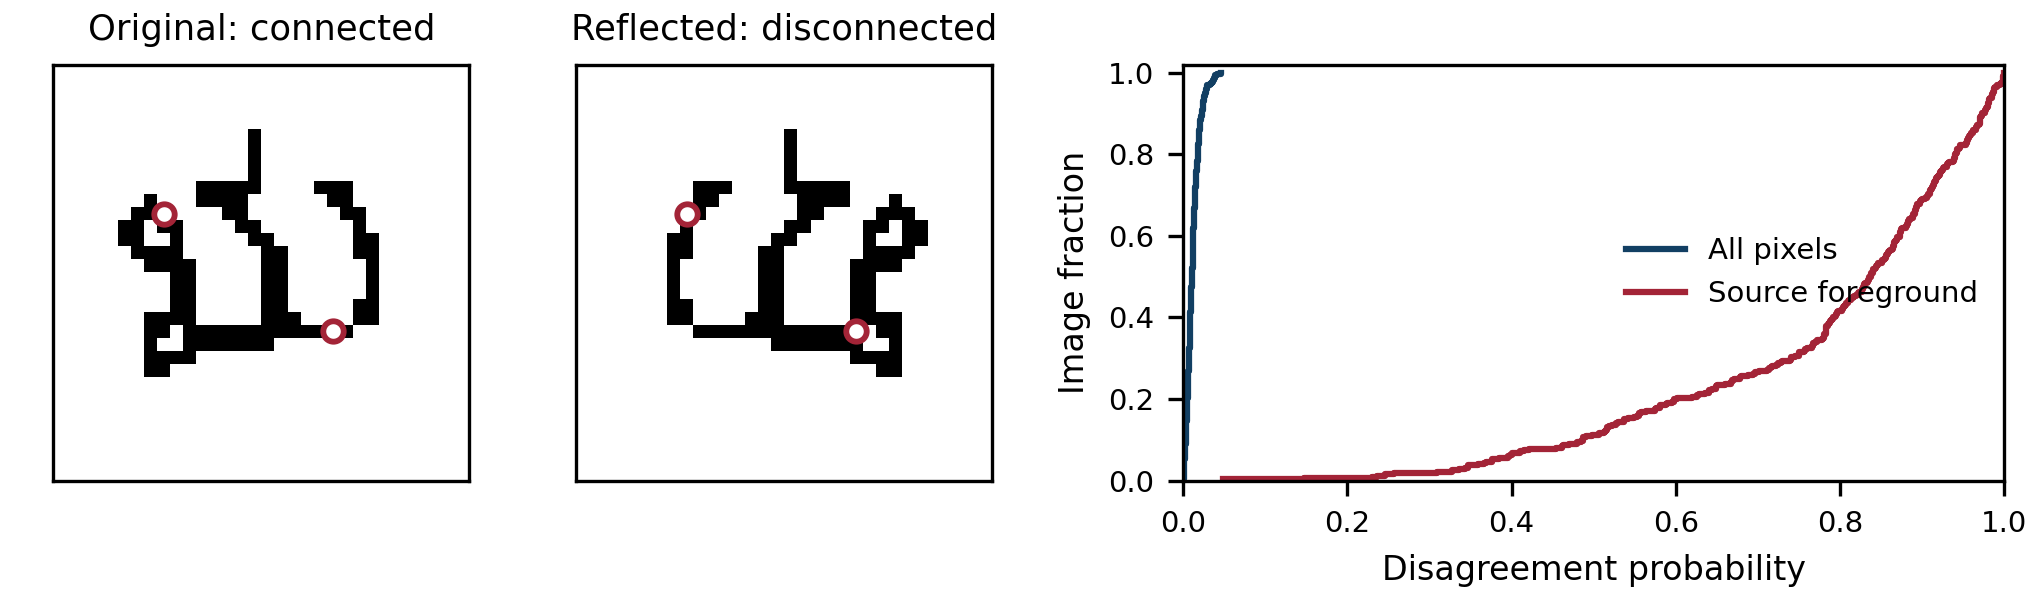
\includegraphics[width=.78\textwidth]{figures/reflection.png}
\caption{A pair of marked foreground pixels is connected in the original glyph and disconnected in its reflection. The distribution functions at right cover all 320 images. The two endpoints of each query stay at the same coordinates across images.}
\label{fig:reflection}\end{figure*}

\section{A Learned Codec Under the Relation Loss}\label{sec:train}
For the learned codec, \eqref{eq:problem} with uniform thresholds is the objective
\begin{align}
 \mathcal L={}&\E[\|X-\hat X\|_2^2/n]
 +\lambda_Q\E|m_{f_X}-m_{f_{\hat X}}|\nonumber\\
 &+\lambda_M\E L_{\rm edge}(X,\tilde Z),
 \label{eq:training}
\end{align}
whose relation term is exact by Proposition~\ref{prop:risk}. One MST per image gives the maximizing vertex of each queried path, which backpropagates \eqref{eq:grad}. Half of the pairs are drawn from the reference foreground. The term $L_{\rm edge}$ compares the MST edge lengths of the source batch and of the equalized codes $\tilde Z$ \cite{moor2020topological}. The encoder and decoder have five convolutions each and a linear output, clipped to $[0,1]$ at evaluation. A sigmoid output saturates at zero on sparse glyphs within twenty steps under the pixel loss, after which the gradient vanishes.

\section{Experiments and Results}
\subsection{Diagram-invariant changes on real glyphs}
We sample 16 official evaluation images from each of the 20 Omniglot evaluation alphabets \cite{lake2015omniglot}, using seed 20261115. Each image is resized to $32\times32$ by nearest-neighbor sampling and black ink is thresholded at gray value 128. Horizontal reflection is a grid automorphism, so by Proposition~\ref{prop:aut} its diagram distance is exactly zero in every degree. The receiver observes the reflected image, and each query applies to the same coordinates as in the source.

We compute the exact uniform-threshold risk without sampling pixel pairs. If $S_i$ and $\hat S_j$ denote foreground components, the number of discordant ordered pairs, with replacement, on an eligible vertex set $A$ is
\begin{align}
 N_A={}&\sum_i |S_i\cap A|^2+\sum_j|\hat S_j\cap A|^2\nonumber\\
 &-2\sum_{ij}|S_i\cap\hat S_j\cap A|^2 .
 \label{eq:count}
\end{align}
Each within-component term counts connected ordered pairs and the last term subtracts the twice-counted intersection. For binary scores any threshold strictly between zero and one activates exactly the foreground. Dividing \eqref{eq:count} by $|A|^2$ gives the exact image-specific disagreement. All 320 glyphs contain foreground after resizing.
\begin{table}[t]\centering
\caption{Exact pair-disagreement probabilities under reflection of 320 evaluation glyphs. Each image receives equal weight.}\label{tab:reflection}
\begin{tabular}{lrrr}\toprule
Eligible endpoints & Mean & Median & Images with error\\\midrule
All pixels & 0.01210 & 0.01102 & 320/320\\
Source foreground & 0.77821 & 0.83633 & 320/320\\\bottomrule
\end{tabular}\end{table}
\begin{table}[t]\centering
\caption{Relation rate in bits per glyph on symmetry orbits of the same 320 glyphs with all-pixel queries. The diagram rate is zero in every column.}\label{tab:orbit}
\begin{tabular}{lrrrr}\toprule
$\delta/\delta_{\max}$ & 0 & 0.1 & 0.25 & 0.5\\\midrule
Reflection pair, $K=2$ & 1.000 & 0.714 & 0.456 & 0.189\\
Dihedral orbit, $K=8$ (mean) & 3.000 & 2.312 & 1.611 & 0.770\\\bottomrule
\end{tabular}\end{table}
Table~\ref{tab:reflection} and Fig.~\ref{fig:reflection} show the dependence on endpoint identity and sampling. Uniform queries are dominated by background pairs for which both answers are zero, and foreground sampling concentrates on stroke relations. These numbers characterize the readout under a known transformation and assume nothing about how often channels produce reflections. Table~\ref{tab:orbit} evaluates Theorem~\ref{thm:orbit} with the same counts. All 320 glyphs have a trivial stabilizer under the eight grid symmetries, and $\delta_{\max}$ has mean 0.01154 and median 0.01049. A receiver restricted to the orbit must obtain 2.31 bits on average to reach one tenth of the zero-rate relation distortion, while no information is needed to match every diagram. On 200 random $5\times5$ templates the closed form agrees with a Blahut--Arimoto solution to within $10^{-15}$ bit.

\subsection{Influence, first-order law and allocation}\label{sec:alloc}
For the same 320 glyphs we compute $\Inf_x(v)$ at every pixel by flipping it and applying \eqref{eq:count} with all pixels eligible. Fig.~\ref{fig:influence} shows the glyph of median total influence. The total $\sum_v\Inf_x(v)$ has mean 0.0826 and median 0.0589 over glyphs. Ink covers 8.4\% of the grid on average and carries 70.8\% of the influence. The ten most influential pixels of a glyph, one percent of the grid, carry 30.9\% of it, and the top five percent carry 65.6\%. The first variation is thus far from the uniform weighting that a pixel error count assumes.
\begin{figure}[t]\centering
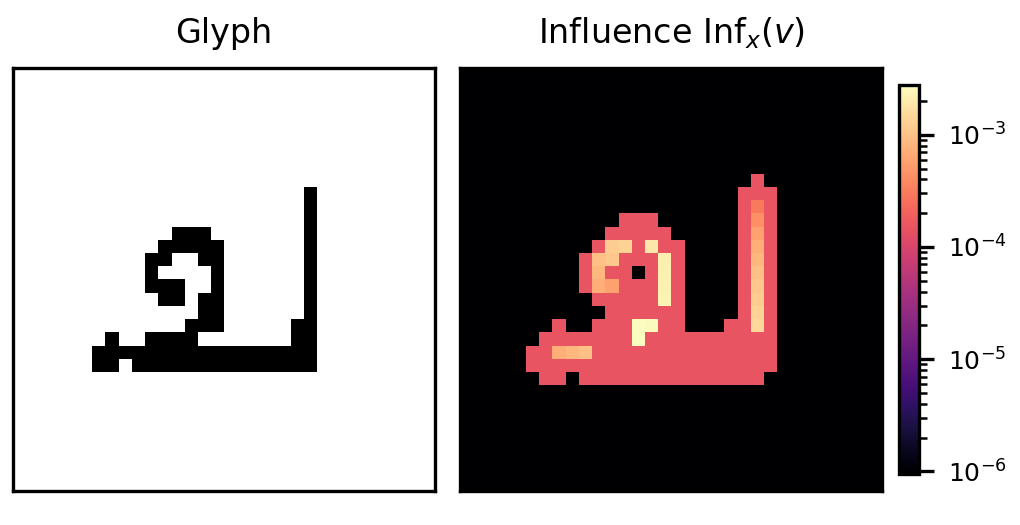
\includegraphics[width=.8\columnwidth]{figures/influence.png}
\caption{A glyph and its exact pixel influences on a logarithmic scale. Cut pixels of the strokes and bridging background pixels dominate.}
\label{fig:influence}\end{figure}

To test \eqref{eq:firstorder} we flip all pixels independently with probability $\varepsilon$ and average the exact risk over 1000, 300 and 100 draws per glyph for $\varepsilon=10^{-4},10^{-3},10^{-2}$. The simulated mean is 0.955, 0.992 and 0.951 times the prediction $\varepsilon\sum_v\Inf_x(v)$. The paired 95\% intervals of the difference contain zero for the first two values and exclude it at $10^{-2}$, where ten flips per image interact. The worst-case remainder $S^2/2$ is not informative at this image size, since $S=1024\,\varepsilon$.

\begin{table}[t]\centering
\caption{Uncoded BPSK transmission of the 320 binary glyphs with uniform power and with the allocation \eqref{eq:lambert}, 100 common noise draws per glyph.}\label{tab:alloc}
\begin{tabular}{crrrrr}\toprule
 & \multicolumn{3}{c}{Relation risk $\times10^{5}$} & \multicolumn{2}{c}{Pixel error $\times10^{3}$}\\\cmidrule(lr){2-4}\cmidrule(lr){5-6}
$E_b/N_0$ & Uniform & Allocated & Ratio & Uniform & Allocated\\\midrule
4 dB & 96.85 & 4.18 & 0.043 & 12.49 & 29.13\\
6 dB & 19.71 & 0.71 & 0.036 & 2.40 & 5.48\\
8 dB & 1.59 & 0.07 & 0.045 & 0.19 & 0.43\\\bottomrule
\end{tabular}\end{table}
Table~\ref{tab:alloc} applies Proposition~\ref{prop:alloc} at the same mean energy per pixel. The allocation lowers the relation risk to about four percent of its uniform-power value and more than doubles the pixel error rate, for which uniform power is optimal. Its power spread within an image averages 7.1, 5.2 and 3.7~dB at the three operating points. The first-order predictions are $3.67\times10^{-5}$, $0.68\times10^{-5}$ and $0.05\times10^{-5}$, and at 8~dB the measured value has a 95\% interval of $[0.03,0.11]\times10^{-5}$. This is a controlled experiment on the readout. The transmitter computes the powers from its own image, the link is uncoded, and the result does not rank learned codecs.

Three controls delimit these results. \emph{An image-independent power map.} One map computed from the mean influence of 200 glyphs of the training alphabets, applied to every evaluation glyph, lowers the relation risk to 46\%, 38\% and 37\% of its uniform-power value at 4, 6 and 8~dB. Most of the gain thus needs the image. The same powers at randomly permuted pixels raise the risk to 2.5--2.8 times the uniform value. \emph{Analog noise outside the half-gap.} On 40 gray $16\times16$ glyph fields with exact all-pair risks, the allocation $p_v\propto c_f(v)^{2/3}$ gives 0.76 times the uniform-power risk at noise deviation $10^{-6}$, against 0.73 predicted by \eqref{eq:l1}. At deviations $10^{-3}$, $10^{-2}$ and 0.1 the ratio is 1.84, 1.08 and 1.12, worse than uniform power, which is why Proposition~\ref{prop:alloc} states no analog rule. \emph{A nontrivial converse.} For each of the 320 glyphs take its eight symmetry images as an equiprobable source and fix three connectivity queries chosen greedily on that orbit. Their answers carry $H_Q=2.48$ bits on average. With the state index sent by three BPSK symbols at 0, 3 and 6~dB, the bound of Theorem~\ref{thm:converse} is 0.98, 1.83 and 2.37 bits, below the 2.16, 2.74 and 2.97 bits that the link carries.

\subsection{Learned codec}\label{sec:neural}
The codec of Section~\ref{sec:train} is trained on 15,700 glyphs of the Omniglot training alphabets at $32\times32$ with $k=410$ ($\rho=0.4$), four power groups of equal power, and a channel and an SNR in $\{0,5,10,15,20\}$~dB drawn per batch. A pixel-loss codec is trained for 100 epochs and then fine-tuned for 20 epochs under four objectives from the same weights: the pixel loss, the relation term ($\lambda_Q=0.01$, 32 images and 128 pairs per batch), the relation and critical-edge terms ($\lambda_M=0.02$), and a TopoJSCC-style sum of cubical and batch Rips diagram distances \cite{erak2026topojscc}. Three seeds are evaluated on 2,048 evaluation glyphs with common noise and 64 fixed pairs per glyph.
\begin{table}[t]\centering
\caption{Learned codec on 2,048 evaluation glyphs, mean of three seeds. Change: paired difference of the risk to the pixel-loss codec in percent, with 95\% interval over glyphs.}\label{tab:neural}
\setlength{\tabcolsep}{3pt}
\begin{tabular}{@{}lccccc@{}}\toprule
 & \multicolumn{2}{c}{Pixel loss} & \multicolumn{3}{c}{Relation term}\\\cmidrule(lr){2-3}\cmidrule(l){4-6}
Channel & PSNR & Risk & PSNR & Risk & Change\\\midrule
AWGN, 0 dB & 24.47 & 0.0550 & 24.43 & 0.0542 & $-1.4$ $[-1.6,-1.3]$\\
AWGN, 10 dB & 27.76 & 0.0369 & 27.68 & 0.0365 & $-1.1$ $[-1.3,-0.8]$\\
AWGN, 20 dB & 28.25 & 0.0348 & 28.17 & 0.0345 & $-0.9$ $[-1.1,-0.6]$\\
Rayleigh, 0 dB & 20.89 & 0.0825 & 20.87 & 0.0807 & $-2.1$ $[-2.3,-2.0]$\\
Rayleigh, 10 dB & 26.02 & 0.0435 & 25.97 & 0.0428 & $-1.6$ $[-1.8,-1.4]$\\
Rayleigh, 20 dB & 27.92 & 0.0358 & 27.84 & 0.0355 & $-1.0$ $[-1.3,-0.8]$\\\bottomrule
\end{tabular}\end{table}
Table~\ref{tab:neural} gives a small effect. The relation term lowers the risk by 0.9 to 2.1\% at a PSNR 0.02 to 0.08~dB below the pixel-loss codec. The intervals exclude zero, but the risk falls in only two of three seeds. Adding the critical-edge term changes the risk by $-0.4$ to $+2.1\%$ and costs a further 0.1~dB. The diagram objective is within 0.1\% of the pixel loss at its default weights. Trained from scratch, a larger $\lambda_Q$ lowers the PSNR and raises the risk it targets (28.0 to 20.0~dB and 0.036 to 0.064 at $\lambda_Q=0.3$ and 10~dB). In this codec the risk follows the reconstruction quality, and the loss buys no protection comparable to Table~\ref{tab:alloc}.

\section{Conclusion}
Connectivity between named locations gives semantic topology a functional with an exact first variation. Near a generic field it is a weighted $\ell^1$ norm whose weights count the location pairs that each pixel connects, and for binary images it is a pixel influence. Diagram functionals are blind to symmetry orbits and to the size of the components that merge, and distinguishing the symmetric images of a template carries a closed-form rate of up to three bits. The converse ties many answers to one channel budget, and the variation gives a closed-form allocation. On real glyphs a few percent of the pixels carry most of the influence, and protecting them lowers the relation risk by more than an order of magnitude at equal energy in an uncoded link, most of which requires powers computed from the image. A learned codec trained with the relation loss gains one to two percent at nearly equal PSNR. Carrying the per-location protection into a compressed representation is the open problem.
\bibliographystyle{IEEEtran}
\bibliography{ref}
\end{document}
